\documentclass{article}
\usepackage{ifthen}
\usepackage{amssymb}
\usepackage{multicol}
\usepackage{graphicx}
\usepackage[absolute]{textpos}
\usepackage{amsmath, amscd, amssymb, amsthm, latexsym}
\usepackage{xspace,rotating,dsfont,ifthen}
\usepackage[spanish,activeacute]{babel}
\usepackage[utf8]{inputenc}
\usepackage{pgfpages}
\usepackage{pgf,pgfarrows,pgfnodes,pgfautomata,pgfheaps,xspace,dsfont}
\usepackage{listings}
\usepackage{multicol}
\usepackage{todonotes}
\usepackage{url}
\usepackage{float}
\usepackage{framed,mdframed}
\usepackage{cancel}

\usepackage[strict]{changepage}


\makeatletter


\newcommand\hfrac[2]{\genfrac{}{}{0pt}{}{#1}{#2}} %\hfrac{}{} es un \frac sin la linea del medio

\newcommand\Wider[2][3em]{% \Wider[3em]{} reduce los m\'argenes
\makebox[\linewidth][c]{%
  \begin{minipage}{\dimexpr\textwidth+#1\relax}
  \raggedright#2
  \end{minipage}%
  }%
}


\@ifclassloaded{beamer}{%
  \newcommand{\tocarEspacios}{%
    \addtolength{\leftskip}{4em}%
    \addtolength{\parindent}{-3em}%
  }%
}
{%
  \usepackage[top=1cm,bottom=2cm,left=1cm,right=1cm]{geometry}%
  \usepackage{color}%
  \newcommand{\tocarEspacios}{%
    \addtolength{\leftskip}{3em}%
    \setlength{\parindent}{0em}%
  }%
}

\usepackage{caratula}
\usepackage{enumerate}
\usepackage{hyperref}
\usepackage{graphicx}
\usepackage{amsfonts}
\usepackage{enumitem}
\usepackage{amsmath}

\decimalpoint
\hypersetup{colorlinks=true, linkcolor=black, urlcolor=blue}
\setlength{\parindent}{0em}
\setlength{\parskip}{0.5em}
\setcounter{tocdepth}{2} % profundidad de indice
\setcounter{section}{3} % nro de section
\renewcommand{\thesubsubsection}{\thesubsection.\Alph{subsubsection}}
\graphicspath{ {images/} }

% End latex config

\begin{document}

\titulo{Práctica 4}
\fecha{2do cuatrimestre 2021}
\materia{Álgebra I}
\integrante{Yago Pajariño}{546/21}{ypajarino@dc.uba.ar}

%Carátula
\maketitle
\newpage

%Indice
\tableofcontents
\newpage

% Aca empieza lo propio del documento
\section{Práctica 4}

Resumen de propiedades de divisibilidad.
\begin{enumerate}
    \item $ \forall d \in \mathbb{Z}: d \neq 0 \implies d|0 $
    \item $ d|a \iff \pm d \vert \pm a \iff |d| \vert |a| $
    \item $ a \neq 0: d|a \implies |d| \leq |a| $
    \item $ Inv(\mathbb{Z} = \{ \pm 1 \}) $
    \item $ d|a \wedge a|d \iff |d| = |a| $
    \item $ a \in \mathbb{Z}; \pm 1 |a \wedge \pm a |a $
    \item $ d|a \wedge d|b \implies d|(a+b) $
    \item $ d|a \implies d|c\cdot a $
    \item $ d|a \wedge d|b \implies d^2 | ab $
\end{enumerate}

\subsection{Ejercicio 1}
\begin{enumerate}
    \item $ ab | c \iff  c= k \cdot ab \implies c = (kb) \cdot a \implies a | c $ Verdadera
    \item $ a^2 = 4k \implies a^2 = 2 \cdot (2k) \implies 2 | a^2 \implies 2 |a $ Verdadera
    \item $ 2 \not \vert a \wedge 2 \not \vert a \implies (2n+1)(2m+1)=2k$. Pero el termino de la izq es impart y el de la dercha par. ABS. Verdadera.
    \item $ 9|3.3 $ pero $ 9 \not \vert 3 $ Falso
    \item $ 2|3+3 $ pero $ 2 \not \vert 3 $ Falso
    \item $ 4|4 \wedge 2|4 $ pero $ 8 \not \vert 4 $ Falso
    \item $ -2|4 $ pero $ -2 > 4 $ Falso
    \item Verdadera. Probado en teórica 10.
    \item Verdadera. $ a|a \implies a |a^2 \implies a|b+a^2-a^2 \implies a|b $
    \item Verdadera. Probado en teórica 10.
\end{enumerate}

\subsection{Ejercicio 2}
\subsubsection{Pregunta i}
\begin{align*}
    3n-1 | n+7 &\implies 3n-1 | 3n-1 \wedge 3n-1 | n+7  \\
    &\implies 3n-1 | (-1)(3n-1) + 3(n+7) \\
    &\implies 3n-1 | -3n+1+3n+21 \\
    &\implies 3n-1 | 22
\end{align*}

Luego $ 3n-1 \in Div_+(22) \iff 3n-1 \in \{ 1,2,11,22 \}$

\begin{enumerate}[label=(\alph*)]
    \item $ 3n-1 = 1 \implies n = \frac{2}{3} \not \in \mathbb{N}$ NO
    \item $ 3n-1 = 2 \implies n = 1 $ luego $ 2|8 $ SI 
    \item $ 3n-1 = 11 \implies n = 4 $ luego $ 11|11 $ SI 
    \item $ 3n-1 = 22 \implies n = \frac{23}{3} \not \in \mathbb{N} $ NO
\end{enumerate}

Rta.: $ n \in \{ 1,4 \} $

\subsubsection{Pregunta ii}
\begin{align*}
    3n-2 | 5n-8 &\implies 3n-2 | 5n-8 \wedge 3n-2 | 3n-2 \\
    &\implies 3n-2 | -3(5n-8) + 5(3n-2) \\
    &\implies 3n-2 | -15n + 24 + 15n - 10 \\
    &\implies 3n-2 | 14
\end{align*}

Luego $ 3n-2 \in Div_+(14) \iff 3n-2 \in \{ 1,2,7,14 \} $

\begin{enumerate}[label=(\alph*)]
    \item $ 3n-2 = 1 \implies n = 1 \in \mathbb{N}$ y además $3n-2 | 5n-8 \iff 1|3$ OK
    \item $ 3n-2 = 2 \implies n = \frac{4}{3} \not \in \mathbb{N}$
    \item $ 3n-2 = 7 \implies n = 3 \in \mathbb{N}$ y además $3n-2 | 5n-8 \iff 7|7$ OK
    \item $ 3n-2 = 14 \implies n = \frac{16}{3} \not \in \mathbb{N}$
\end{enumerate}

Rta.: $n = 1$ y $n = 3$

\subsubsection{Pregunta iii}
\begin{align*}
    2n+1 | n^2+5 &\implies 2n+1 | n^2+5 \wedge 2n+1 | 2n+1 \\
    &\implies 2n+1 | 2(n^2+5) + (-n)(2n+1) \\
    &\implies 2n+1 | 10-n \wedge 2n+1 | 2n+1 \\
    &\implies 2n+1 | 2(10-n) + 2n+1 \\
    &\implies 2n+1 | 21
\end{align*}
  
Luego $ 2n+1 \in Div_+(21) \iff 2n+1 \in \{ 1,3,7,21 \}$

\begin{enumerate}[label=(\alph*)]
    \item $2n+1 = 1 \implies n = 0 \not \in \mathbb{N}$
    \item $2n+1 = 3 \implies n = 1 $ y $ 3|6 $
    \item $2n+1 = 7 \implies n = 3 $ y $ 7|14 $
    \item $2n+1 = 21 \implies n = 10 $ y $ 21|105 $
\end{enumerate}

Rta.: $ n \in \{ 1,3,10 \} $

\subsubsection{Pregunta iv}
\begin{align*}
    n-2 | n^3-8 &\implies n-2 | n^3-8 \wedge n-2 | n-2 \\
    &\implies n-2 | n^3-8 +(-n^2)(n-2) \\
    &\implies n-2 | n^3 - 8 -n^3 + 2n^2 \\
    &\implies n-2 | - 8 + 2n^2 \wedge n-2 | n-2 \\
    &\implies n-2 | 2n^2 - 8 + (-2n)(n-2) \\
    &\implies n-2 | 2n^2 - 8 + -2n^2 + 4n \\
    &\implies n-2 | - 8 + 4n \wedge n-2 | n-2 \\
    &\implies n-2 | - 8 + 4n -4n+8 \\
    &\implies n-2 | 0 \\
\end{align*}

Rta.: $ n \in \mathbb{N} $

\subsection{Ejercicio 3}
\subsubsection{Pregunta i}
Demostración por inducción.

Defino $ p(n): a-b | a^n-b^n; \forall n \in \mathbb{N} $

\textbf{Caso base n=1}

$ p(1): a-b | a-b \iff a-b = k(a-b); k \in \mathbb{Z} $

Dado que $ k = 1 $ lo cumple, $ p(1) $ es verdadero.

\textbf{Paso inductivo}

Dado $ k \geq 1 $ quiero probar que $ p(k) \implies p(k+1) $

HI: $ a-b | a^k-b^k $

Qpq: $ a-b | a^{k+1}-b^{k+1} \iff a-b | a^k \cdot a - b^k \cdot b $

Por ejercicio 8 de la guía 2: $ a^n - b^n = (a-b) \cdot \sum_{i=1}^{n}\cdot a^{i-1}\cdot b^{n-i} $

Es decir, existe $ x \in \mathbb{Z} $ tal que $ a^n - b^n = (a-b) \cdot x $ como se quería probar.

Luego $p(n)$ es verdadero $ \forall n \in \mathbb{N} $

\subsubsection{Pregunta ii}
$ a+b = a - (-b) \implies a - (-b) | a^n - (-b)^n \implies a+b | a^n - b^n$

\subsubsection{Pregunta iii}
$ a+b = a-(-b) \implies a-(-b)|a^n - (-b)^n \implies a+b | a^n + b^n $

\subsection{Ejercicio 4}
Por inducción.

Defino $ p(n): 2^{n+2}|a^{2^n}-1; \forall n \in \mathbb{N} $

\textbf{Caso base n=1}

$ p(1): 2^{1+2}|a^{2^1}-1 \iff 2^3 | a^{2}-1 \iff 8 | a^{2}-1 $

Se que a es un entero immpar, luego $ a = 2k + 1; k \in \mathbb{Z} $

Por lo tanto,
\begin{align*}
    8 | a^{2}-1 &\iff 8 | (2k + 1)^{2}-1 \\
    &\iff 8 | 4k^4 + 4k + 1 - 1 \\
    &\implies 8 | 4k^2 + 4k \\
    &\implies 8 | 4(k^2 + k) \\
    &\iff 4(k^2 + k) = 8\cdot m; m \in \mathbb{Z} \\
    &\iff k^2 + k = 2\cdot m \\
    &\iff k(k+1) = 2\cdot m \\
\end{align*}

Que es verdadero pues el producto de par e impar es siempre verdadero.

\textbf{Paso inductivo}

Dado $ k \geq 1 $ quiero probar que $ p(k) \implies p(k+1) $

HI: $ 2^{k+2}|a^{2^k}-1 $

Qpq: $ 2^{k+3}|a^{2^{k+1}}-1 $

Pero,
\begin{align*}
    2^{k+2} | a^{2^k}-1 &\implies 2^{k+3} | 2(a^{2^k}-1) \\
    &\implies 2^{k+4} | 2(a^{2^k}-1)(a^{2^k}+1) \\
    &\implies 2^{k+4} | 2(a^{2^{k+1}}-1) \\
    &\implies 2^{k+3} | a^{2^{k+1}}-1 \\
\end{align*}

Luego $p(n)$ es verdadero, $ \forall n \in \mathbb{N} $

\subsection{Ejercicio 5}
\subsubsection{Pregunta i}
Como n es compuesto: n=kq con $1<k<n, 1<q<n$ \\
$2^{n}-1=2^{kq}-1=[2^{k}]^{q}-1$ \\
Usando el resultado del ejercicio 3.i: $a-b | a^n-b^n$ \\
$2^k-1 | (2^{k})^{q}-1^q$ O puesto de otra forma: $2^k-1 | 2^n-1$ \\
$1 < 2^k-1 < 2^n-1$ \\
Luego, como $2^{n}-1$ tiene un divisor no trivial (distinto de $\pm1, \pm(2^{n}-1)$) concluyo que es compuesto.
\subsubsection{Pregunta ii}
"Probar que si $2^{n}+1$ es primo, entonces n es una potencia de 2."

Voy por el absurdo: supongo que n no es una potencia de 2 $\implies 2^{n}+1$ es compuesto

Si n no es una potencia de 2 se puede escribir como:

$n = 2^{j}k$ con k impar $\geq 1$, j$\geq 0$ \\
$2^{n}+1=2^{2^jk}+1=(2^{2^j})^k+1^k=(2^{2^j})^k-(-1)^k$ porque k es impar \\
Puedo volver a usar la propiedad: $a-b | a^n-b^n$ \\
$2^{2^j}+1 | (2^{2^j})^k-(-1)^k$ \\
$1 < 2^{2^j}+1 < 2^{n}+1 \implies 2^{n}+1$ es compuesto \\
Luego $2^{n}+1$ es primo $\implies$ n es una potencia de 2.

\subsection{Ejercicio 6}
\subsubsection{Pregunta i}
$ n! | \prod_{i = n_0}^{n_0 + n - 1} \iff \prod_{i = n_0}^{n_0 + n - 1} = k\cdot n!$

Pero,
\begin{align*}
    \prod_{i = n_0}^{n_0 + n - 1} &= n_0 \cdot (n_0 +1) \cdot ... \cdot (n_0 + n - 2) \cdot (n_0 + n -1) \\
    &= \frac{(n_0+n-1)!}{(n_0-1)!}
\end{align*}

Recordando el número combinatorio, 

$ \prod_{i = n_0}^{n_0 + n - 1} = \binom{n_0+n-1}{n} \cdot n! $

Y dado que el combinatorio $ \in \mathbb{Z} $, $ n! | \prod_{i = n_0}^{n_0 + n - 1} $ como se quería probar.

\subsubsection{Pregunta ii}
\begin{align*}
    2 | \binom{2n}{n} &\iff 2|\frac{2n!}{n!\cdot n!} \\
    &\iff \frac{2n!}{n!\cdot n!} = 2k \\
    &\iff \frac{2n \cdot (2n-1)!}{n!\cdot n!} = 2k \\
    &\iff \frac{n \cdot (2n-1)!}{n!\cdot n!} = k \\
\end{align*}

Luego debo probar que $k \in \mathbb{Z}$
\begin{align*}
    k \in \mathbb{Z} &\iff n!\cdot n! | n \cdot (2n-1)! \\
    &\iff n! | \frac{(2n-1)!}{(n-1)!} \\
\end{align*}

Por ejercicio 6.1 esto se cumple, por lo tanto $ k \in \mathbb{Z} $ como se quería probar.

Y así, $\binom{2n}{n}$ es divisible por 2.

\subsection{Ejercicio 7}
\subsubsection{Pregunta i}
\begin{align*}
    99 | 10^{2n} + 197 &\iff 10^{2n} \equiv -197(99) \equiv 1(99) \\
    &\iff 100^{n} \equiv 1(99) \iff 1^n \equiv 1(99) \iff 1 \equiv 1(99) \\
\end{align*}
Que es verdadero, $ \forall n \in \mathbb{N} $

\subsubsection{Pregunta ii}
\begin{align*}
    9| 7\cdot 5^{2n} + 2^{4n+1} &\iff 7\cdot 25^n + 2\cdot 16^n \equiv 0(9) \\
    &\iff 7\cdot 16^n + 2\cdot 16^n \equiv 0(9) \\
    &\iff 16^n \cdot 9 \equiv 0(9) \\
    &\iff 16^n \cdot 0 \equiv 0(9) \\
    &\iff 0 \equiv 0(9) \\
\end{align*}
Que es verdadero, $ \forall n \in \mathbb{N} $

\subsubsection{Pregunta iii}
\begin{align*}
    56 | 13^{2n} + 28 \cdot n^2 - 84n -1 &\iff 13^{2n} + 28n^2 + 84n \equiv 1 (56) \\
    &\iff 1^{n} + 28n^2 + 28n \equiv 1 (56) \\
    &\iff 28(n^2+n)\equiv 0 (56) \\
    &\iff 2\cdot 28(n^2+n)\equiv 2\cdot 0 (56) \\
    &\iff 56(n^2+n)\equiv 0 (56) \\
    &\iff 0(n^2+n)\equiv 0 (56) \\
    &\iff 0\equiv 0 (56) \\
\end{align*}
Que es verdadero, $ \forall n \in \mathbb{N} $

\subsubsection{Pregunta iv}
TODO

\subsection{Ejercicio 8}
\begin{enumerate}
    \item $ 133 = (-9) \cdot (-14) + 7 $ 
    \item $ 13 = 0 \cdot 111 + 13 $ 
    \item $\begin{cases}
        c = 4; r = (b-7) & 1\leq b \leq 7 \\
        c = 3; r = 7 & \text{otherwise} 
    \end{cases}$
    \item TODO
    \item TODO
    \item TODO
\end{enumerate}

\subsection{Ejercicio 9}
Se que $ a \equiv 5 (18) $

\begin{enumerate}
    \item $ a^2 - 3a + 11 \equiv 5^2 - 15 + 11 \equiv 25 + 3 + 11 \equiv 3(18) $
    \item $ a\equiv 5(18) \implies a \equiv 5(3) \iff a\equiv 2(3) $
    \item $ a\equiv 5(18) \implies a \equiv 5(9) $ luego $ 4a+1 \equiv 4.5 + 1 \equiv 21 \equiv 3(9) $
    \item Se que $ a \equiv 5(18) \implies a = 18k + 5$
    \begin{align*}
        7a^2 + 12 &= 7(18k + 5)^2 + 12 \\
        &= 7\cdot (324k^2 + 180k+ 25) + 12 \\
        &= 2268k^2 + 1260k+ 175 + 12 \\
        &= 2268k^2 + 1260k+ 187 \\
        &\equiv 0k^2 + 0k+ 19 \equiv 19(28) \\
    \end{align*}
\end{enumerate}

\subsection{Ejercicio 10}
\subsubsection{Pregunta i}
$ a\equiv 22 \equiv 8(14)$

$ a\equiv 8(14) \implies a \equiv 8(7) \equiv 1(7)$

$ a\equiv 8(14) \implies a \equiv 8(2) \equiv 0(2)$

\subsubsection{Pregunta ii}
$ a \equiv 13 \equiv 3(5) $

$ 33a^3 + 3a^2 - 197a +5 \equiv 3 \cdot 3^3 + 3 \cdot 3^2 - 197 \cdot 3 + 5 \equiv 3.2 + 3.4 -2.3 + 2 \equiv 4(5) $

\subsubsection{Pregunta iii}
Pruebo con algunos casos:
\begin{enumerate}
    \item n = 1: $ S(1) = -1 $ 
    \item n = 2: $ S(2) = -1 + 2 = 1 $ 
    \item n = 3: $ S(3) = -1 + 2 -6 = -5 $ 
    \item n = 4: $ S(4) = -1 + 2 -6 + 24 = 19 \equiv 7(12) $ 
    \item n = 5: $ S(5) = -1 + 2 -6 + 24 -120 = -101 \equiv 7(12) $ 
\end{enumerate}

Veo que a partir de n = 4, la congruencia es igual a cero. Pues en el factorial encuentro $ n.(n-1)....4.3... $

Por lo tanto $r_{12}(S(n\geq 4))$ = 7

Asi, los posibles restos son:
\begin{enumerate}
    \item n = 1. $ r_{12}(S(1)) = 11 $
    \item n = 2. $ r_{12}(S(2)) = 1 $
    \item n = 3. $ r_{12}(S(3)) = 7 $
    \item n = 4. $ r_{12}(S(4)) = 7 $
\end{enumerate}

\subsection{Ejercicio 11}
Estos ejercicios se resuelven con tablas de restos de forma trivial.

\subsubsection{Pregunta i}
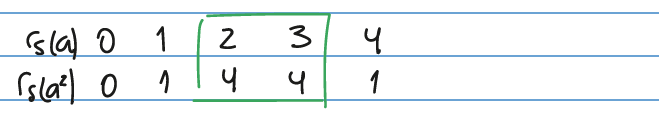
\includegraphics[width=300px]{4.11.1}

\subsubsection{Pregunta ii}
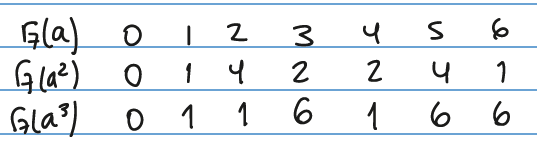
\includegraphics[width=300px]{4.11.2}

No existe a tal que $ r_3(a^3) = 4$

\subsubsection{Pregunta iii}
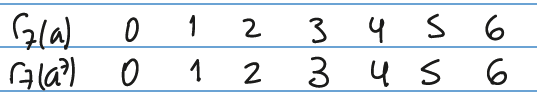
\includegraphics[width=300px]{4.11.3}

\subsubsection{Pregunta iv}
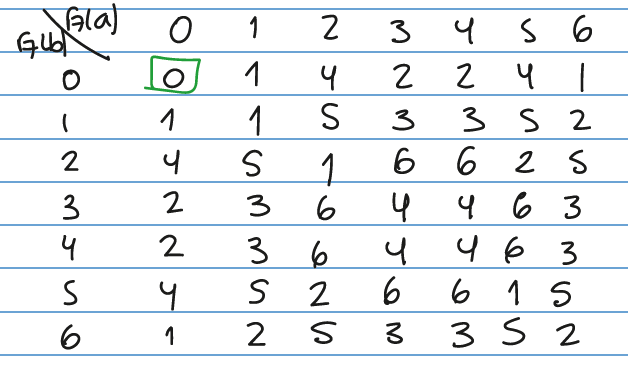
\includegraphics[width=300px]{4.11.4}

\subsubsection{Pregunta v}
TODO

\subsection{Ejercicio 12}
\begin{enumerate}
    \item $ 2^{5k} \equiv 1(31) \implies 32^k \equiv 1^k \equiv 1(31)$
    \item $ 2^{51833} \equiv 2^{5\cdot 10366 + 3} \equiv (2^5)^{10366} \cdot 2^3 \equiv 1^{10366} \cdot 8 \equiv 8 (31) $
    \item $ 2^k \equiv 8(31) \iff 2^{5k+n} \equiv 8(31) \iff 1^k \cdot 2^n \equiv 8(31) \iff 2^n \equiv 8 (31) \implies n = 3 = r_5(k) $
    \item $ 43 \cdot 2^{163} + 11 \cdot 5^{221} + 61^{999} \equiv 12 \cdot 8 + 11\cdot 25 + (-1)^{999} \equiv 3 + 27 -1 \equiv 29(31)$
\end{enumerate}

\subsection{Ejercicio 13}
Por inducción.

Defino $ p(n): a_n \equiv 3^n(7); \forall n \in \mathbb{N} $

\textbf{Casos base n = 1; n = 2}

$ p(1): a_1 \equiv 3^1(7) \equiv 3(7) $

$ p(2): a_2 \equiv 3^2(7) \equiv 2(7) \equiv -5(7)$

Luego $ p(1); p(2) $ son verdaderas.

\textbf{Paso inductivo}
Dado $ k\geq 2 $ quiero probar que $ (p(k) \wedge p(k+1)) \implies p(k+2) $

HI: $a_k \equiv 3^k(7)$ y $a_{k+1} \equiv 3^{k+1}(7)$

Qpq: $a_{k+2} \equiv 3^{k+2}(7) \iff a_{k+2} \equiv 3^k \cdot 9 \equiv 3^k \cdot 2 $

Pero,
\begin{align*}
    a_{k+2} &= a_{k+1} - 6^{2k} \cdot a_k + 21^k \cdot k^{21} \\ 
    &\equiv 3^{k+1} - 6^{2k} \cdot 3^k + 21^k \cdot k^{21} (7)\\ 
    &\equiv 3^k \cdot 3 - 3^k (7)\\ 
    &\equiv 3^k \cdot (3 - 1) (7)\\ 
    &\equiv 3^k \cdot 2 (7)\\ 
\end{align*}

Luego $ (p(k) \wedge p(k+1)) \implies p(k+2) $ y por lo tanto $ p(n) $ es verdadero, $ \forall n \in \mathbb{N} $

\subsection{Ejercicio 14}
\subsubsection{Pregunta i}
\begin{enumerate}
    \item $ 1365 = (0101010101)_2$
    \item $ 2800 = (101011110000)_2$
    \item $ 2\cdot 2^{13} = (110000000000000)_2$
    \item TODO
\end{enumerate}

\subsubsection{Pregunta ii}
\begin{align*}
    2800 &= 175 \cdot 16 + \textbf{0} \\
    175 &= 10 \cdot 16 + \textbf{15} \\
    10 &= 0 \cdot 16 + \textbf{10} \\
\end{align*}

$ 2800 = (AF0)_{16}$

\subsection{Ejercicio 15}
Multiplicar por dos a un número binario, hace que se sume uno al exponente de cada término (pensando como la sumatoria decimal de potencias de 2)

En la secuencia binaria, esto hace que se corran hacia la izq los digitos.

La división por dos hace lo mismo pero restando, generando un corrimiento hacia la derecha.

\subsection{Ejercicio 16}
Para demostrar los criterios de divisibilidad defino $ D = r_n \cdot 10^n + r_{n-1}\cdot 10^{n-1}+...+r_1 \cdot 10 + r_0 $ el desarrollo decimal de un número entero positivo.

\subsubsection{Divisiblidad por 8}
$ D \equiv r_n \cdot 2^n + r_{n-1}\cdot 2^{n-1}+...+r_1 \cdot 2 + r_0 (8)$

Se que $ 2^3 \equiv 0 (8) $ luego todos los términos de D con $ n \geq 3 $ van a ser congruentes a 0 mod 8.

Luego $ D \equiv r_2 \cdot 2^2 + r_1 \cdot 2 + r_0 \equiv r_2 \cdot 4 + r_1 \cdot 2 + r_0 $

Por lo tanto $ 8|D \iff d_2 \cdot 4 + d_1 \cdot 2 + d_0 \equiv 0(8) $ con $d_i$ es i-ésimo digito de der a izq.

\subsubsection{Divisiblidad por 9}
$ D \equiv r_n \cdot 1^n + r_{n-1}\cdot 1^{n-1}+...+r_1 \cdot 1 + r_0 (9)$ \\
$ D \equiv r_n + r_{n-1} +...+ r_1 + r_0 (9)$

Es decir que $ 9|D \iff \sum_{i=0}^{n}d_i \equiv 0(9)$

Coloquialmente, la suma de los dígitos de D es divisible por 9.

\subsection{Ejercicio 17}
\subsubsection{Pregunta i}
\begin{align*}
    k = (aaaa)_7 &\implies k = a\cdot 7^3 + a\cdot 7^2 + a \cdot 7 + a \\
    &\implies k = a(7^3+7^2+7+1) \\
    &\implies k \equiv a(7+1+7+1)(8) \\
    &\implies k \equiv 16a \equiv 0(8) \\
\end{align*}

\subsubsection{Pregunta ii}
Para $ d \equiv 0 (2) $ pues las potencias impares de 7 $ \implies 7^{2n+1}\equiv 7 (8) $ y las pares $ \implies 7^{2n}\equiv 1 (8) $

Así, $ 1+7= 8 \equiv 0(8) \iff 8|k $

\subsection{Ejercicio 18}
\begin{enumerate}
    \item $ (2532:63) = 3 $ y $ 3 = -5 \cdot 2532 + 201 \cdot 63$
    \item $ (131:23) = 1 $ y $ 1 = -10 \cdot 131 + 57 \cdot 23$
    \item TODO
\end{enumerate}

\subsection{Ejercicio 19}
Por algoritmo de Euclides se que $ (a:b) = (b:r_b(a)) $ 

Luego $(a:b) = (b:27) \iff (a:b) = (27:r_{27}(b)) = (27:21) = 3$

\subsection{Ejercicio 20}
\subsubsection{Pregunta i}
Sea d tal que $ (5a+8:7a+3) = d $

Por propiedades del MCD se que: $ (d|5a+8) \wedge (d|7a+3) \iff d|7(5a+8) - 5(7a+3) \iff d|35a+56-35a-15 \iff d|41$

Luego $ d \in Div_+(41) \iff d \in \{ 1,41 \} $ como se quería probar.

a = 1 $ \implies (13:10) = 1 $
a = 23 $ \implies (123:164) = 41 $

\subsubsection{Pregunta ii}
Sea d tal que $ (2a^2+3a-1:5a+6) = d $

Por propiedades del MCD se que: $ (d|2a^2+3a-1) \wedge (d|5a+6) \implies d|5(2a^2+3a-1) - 2(5a+6) \iff d|3a-5 \implies d|-5(3a-5)+3(5a+6)
\iff d|-15a+25+15a+18 \iff d|43 $


Luego $ d\in Div_+(43) \iff d \in \{ 1,43 \} $ como se quería probar.

a = 1 $ \implies (4:11) = 1 $
a = 16 $ \implies (559:86) = 43 $

\subsubsection{Pregunta iii}
Sea d tal que $ (a^2-3a+2:3a^3-5a^2) = d $

Usando el algoritmo de Euclides, $ d = (a^2-3a+2:6a-8) $

Luego $ (d|a^2-3a+2) \wedge (d|6a-8) \implies d|6a^2-18a+12-6a^2+8a \implies d|-10a+12 \implies d|-30a+36+30a-40 \implies d|4$

Por lo tanto $ d \in Div_+(4) \iff d \in \{ 1,2,4 \} $

Pero $ \forall a: (a^2-3a+2 \equiv 0 (2)) \wedge (3a^3-5a^2 \equiv 0 (2))$. Luego $d \neq 1$

Así $ d \in \{ 2,4 \}$

a = 1 $ \implies (0:-2) = 2 $
a = 2 $ \implies (0:4) = 4 $

\subsection{Ejercicio 21}
Por enunciado se que $ (a:b) = 1 \implies 1 = s.a + t.b$  $s,t \in \mathbb{Z}$

Sea $ d = (7a-3b:2a-b) $

Se que $ (d| 7a-3b) \wedge (d|2a-b) \implies d|7a-3b-6a+3b \implies d|a $

De igual manera $ (d| 7a-3b) \wedge (d|2a-b) \implies d|14a-6b-14a+7b \implies d|b $

Luego $ (d|a \wedge d|b) \implies (d|s.a \wedge d|t.b) \implies d|s.a + t.b \implies d|1$

Pero $ d|1 \iff d=1 $

Por lo tanto $ d=1 \implies 7a-3b \perp 2a-b $ como se quería probar.

\subsection{Ejercicio 22}
Por enunciado se que $ (a:b) = 2 $. Sea $ d = (7a+3b:4a-5b) $

\textbf{Corpimizar}

Por propiedades del MCD $ a = 2\cdot a' $; $ b = 2b' $ con $ a' \perp b' $

\begin{align*}
    d &= (7\cdot (2a') + 3\cdot(2b'):4 \cdot (2a')-5\cdot (2b')) \\
    &= (14a' + 6b':8a' - 10b') \\
    &= (2\cdot (7a' + 3b'):2\cdot (4a' - 5b')) \\
    &= 2 \cdot (7a' + 3b':4a' - 5b') \\
\end{align*}

Defino $ k = (7a' + 3b':4a' - 5b') $

$ (k|7a' + 3b') \wedge (k|4a' - 5b') \implies k|28a' + 12b' -28a' +35b' \implies k|47b' $

$ (k|7a' + 3b') \wedge (k|4a' - 5b') \implies k|35a'+15b'+12a'-15b' \implies k|47a' $

Rdo.: $ k|a \wedge k|b \iff k|(a:b)$

Luego $ k|47a' \wedge k|47b' \iff k|(47a':47b') \implies k|47(a':b') \iff k|47 $

Así, $ k \in Div_+(47) \iff k\in \{ 1,47 \} $

k = 1 $ \implies d = 2.1 = 2 $ \\
k = 1 $ \implies d = 2.47 = 94 $

a = 0, b = 2 $ \implies (6:-10) = 2$
a = 26, b = 2 $ \implies (188:94) = 2$

\subsection{Ejercicio 23}
\subsubsection{Pregunta i}

$ \frac{b+4}{a} + \frac{5}{b} = \frac{b(b+4) + 5a}{ab} = c $

Luego $ c\in \mathbb{Z} \iff ab|b^2+4b+5a $ con $ a\perp b $

Rdo.: Sean $ c \perp d: c|a \wedge d|a \iff cd|a $

Entonces, $ (a|b^2+4b+5a) \wedge (b|b^2+4b+5a) \iff (a|b^2+4b) \wedge (b|5a) \iff (a|b(b+4)) \wedge (b|5)
\iff (a|b+4) \wedge (b|5) $

Luego $ b \in Div(5) \iff b \in \{ \pm 1, \pm 5 \} $

$ b=1 \implies a|5 \implies a \in \{ \pm 1, \pm 5 \}$ \\
$ b=-1 \implies a|3 \implies a \in \{ \pm 1, \pm 3 \}$ \\
$ b=5 \implies a|9 \implies a \in \{ \pm 1, \pm 3, \pm 9 \}$ \\
$ b=-5 \implies a|-1 \implies a \in \{ \pm 1 \}$

\subsubsection{Pregunta ii}
$ \frac{9a}{b} + \frac{7a^2}{b^2} = \frac{9ab + 7a^2}{b^2} \implies b^2|9ab + 7a^2 $

Luego $ b|9ab + 7a^2 \iff b|a(9b+7a) \implies b|9b+7a \iff b|7a \iff b|7 $

Así, $ b \in \{ \pm 1, \pm 7 \} $

$ b = \pm 1 $ cumple lo pedido.

$ b = 7 \implies 49|9.7.a+7.a^2 \iff 49|7(9a+a^2) \implies 7|9a+a^2 \implies 7|a(9+a) \implies 7|9+a 
\implies 9+a = 7k \iff a \equiv -9 \equiv 5(7) $

$ b = -7 \implies 49|9.(-7).a+7a^2 \implies 49|7(-9a+a^2) \implies 7|-9a+a^2 \implies 7|a(-9+a) \implies 7|-9+a 
\implies -9+a = 7k \iff a \equiv 9 \equiv 2 (7)$

Rta.: \\
$b = 1, a \in \mathbb{Z} \vee \\b = -1, a \in \mathbb{Z} \vee \\b = 7, a \equiv 5(7) \vee \\b = -7, a \equiv 2(7)$

\subsection{Ejercicio 24}
TODO

\subsection{Ejercicio 25}
\subsubsection{Pregunta i}
$ p|\binom{9}{k} \iff p|\frac{p!}{k! \cdot (p-k)!} \implies \frac{p(p-1)!}{k! \cdot (p-k)!} \equiv 0(p)$

Como se quería probar.

\subsubsection{Pregunta ii}
Usando el resultado del inciso anterior,

\begin{align*}
    (a+b)^p &= \binom{p}{1}a^p \cdot b^0 + \binom{p}{2}a^{p-1} \cdot b^1 ... + \binom{p}{p}a^0 \cdot b^p \\
    &\equiv a^p + 0 \cdot b^1 + 0 + 0 + ... + b^p (p) \\
    &\equiv a^p + b^p (p)\\
\end{align*}

Como se quería probar.

\subsection{Ejercicio 26}
\subsubsection{Pregunta i}

$ a^2 = 3b^3 \implies 3|a^2 \implies 3|a \iff a \equiv 0(3)$

Luego $ a = 9 \implies a^2 = 81 \implies 81 = 3.27 = 3.3^3$  

Así, $ a = 9; b = 3 $ cumplen lo pedido.

\subsubsection{Pregunta ii}
$ 7a^2 = 8b^2 $

Por TFA la factorización en primos de $ 7a^2 $ tiene que ser igual a la de $ 8b^2 $

Luego $ 2^k | a \implies 2^{2k} | a^2 $

Es decir que el factor 2 en $ 7a^2 $ tiene exponente par, luego $ 8b^2 $ debe tener factor 2 con multiplicidad par.

Pero $ 8b^2 = 2^3 \cdot b^2 \implies $ 2 no puede tener multiplicidad par.

Luego, $ \not \exists a,b \in \mathbb{Z}: 7a^2 = 8b^2 $

\subsection{Ejercicio 27}
Quiero probar que $ \sqrt[n]{p} \not \in Q$

Por el absurdo, supongo que $ \sqrt[n]{p} = \frac{a}{b} $

Luego, $ \sqrt[n]{p} = \frac{a}{b} \iff p \cdot b^n = a^n $

Pero si miro la factorización de ambos terminos de la igualdad:

Con n par: En $ p.b^n $ el factor p tendrá exponente impar, mientras que en $ a^n $ tendrá exponente par.

Con n impar: $ n = 2k+1 $ En $ p.b^{2k+1} $ el factor p tendrá exponente par, mientras que en $ a^{2k+1} $ tendrá exponente impar.

En ambos casos se llega a un absurdo y así queda demostrado que $ \sqrt[n]{p} \not \in Q; n\geq 2; p \text{ primo} $

\subsection{Ejercicio 28}
$ pq|a^n \implies p|a^n \wedge q|a^n $ pues $ p\in fact(a^n) $ y $ q\in fact(a^n) $

Luego la factorización de $ a^n $ será de la forma $ a^n = p^{n.r_1} \cdot q^{n.r_2} \cdot ... $

Pero la factorización de a será $ a = a^n = p^{r_1} \cdot q^{r_2} \cdot ... $ y en particular $ a = p.q(p^r_1-1 \cdot q^r_2-1 \cdot ...) $

Luego $ pq|a $ como se quería probar.

\subsection{Ejercicio 29}
Rdo.: Sea $ a = p_1^{r_1} \cdot p_n^{r_n}$ con $p_i$ primo, $ Div_+(a) = (r_1 + 1)...(r_n + 1) $

\begin{enumerate}
    \item $ 9000 = 2^3.3^3.5^3 \implies \#Div_+ = (3+1)(2+1)(3+1) = 48$
    \item $ 15^4.42^3.56^2 = 2^9.3^7.5^4.7^5 \implies \#Div_+ = (9+1)(7+1)(4+1)(5+1) = 2400 $ 
    \item $ 10^n.11^{n+1} = 2^n.5^n.11^n \implies \#Div_+ = (n+1)(n+1)(n+2) = n^3 + 4n^2+6n+2$ 
\end{enumerate}

\subsection{Ejercicio 30}
\subsubsection{Pregunta i}

$ a = 2^4.5^123 $

Los $ Div_+(a) $ serán de la forma $ 2^i . 5^j $ con $ 0\leq i \leq 4 $ y $ 0\leq j \leq 123 $

Luego $ \sum_{i=0}^{4}\left( \sum_{j=0}^{123}2^i.5^j \right) = \left( \sum_{i=0}^{4}2^i \right) \cdot \left( \sum_{j=0}^{123}5^j \right) = \frac{2^5 - 1}{1} \cdot \frac{5^124 - 1}{4} $

\subsubsection{Pregunta ii}
$ a = 10^n \cdot 11^{n+1} $

Los $ Div_+(a) $ serán de la forma $ 2^i . 5^j . 11^k $ con $ 0\leq i \leq n $ y $ 0\leq j \leq n $ y $ 0\leq k \leq n+1 $

Luego $ \sum_{i=0}^{n}\left( \sum_{j=0}^{n} \left( \sum_{k=0}^{n+1} 2^i.5^j.11^k \right) \right) = \left( \sum_{i=0}^{n}2^i \right) \cdot \left( \sum_{j=0}^{n}5^j \right) \cdot \left( \sum_{k=0}^{n+1}11^k \right) = (2^{n+1} - 1)(\frac{5^{n+1}-1}{4})(\frac{11^{n+2}-1}{10})$

\subsection{Ejercicio 31}
$ 6552 = 2^3.3^2.7.13 $

Busco n tal que $ 6552 . n = k^2 \iff (2^3.3^2.7.13).n = k^2 $

Luego los factores primos de $ k^2 $ deben ser potencias de 2.

$ n = 2.7.13 \implies k^2 = 2^4.3^2.7^2.13^2 $ que efectivamente es $ (4.3.7.13)^2 = 1092 = 1192464 = 2^4.3^2.7^2.13^2 $

Luego $ n = 182 $ es el menor $ n \in \mathbb{N} $ que cumple lo pedido.

\subsection{Ejercicio 32}
$ab$ es un cuadrado si $ ab = (p_1^{n_1}...p_k^{n_k})^2 $

Si $ (a:b) = 1 \implies $ a y b no tienen primos en común.

Pero por enunciado, a y b son cuadrados, luego deben tener factorización en primos de la forma $ a = p_1^{2k_1} \cdot ... p_n^{2k_n} $

Y por lo tanto, $ a = (p_1^{k_1} \cdot ... p_n^{k_n})^2 $. Lo mismo con b, como se quería probar.

\subsection{Ejercicio 33}
\subsubsection{Pregunta i}

$ 945 = 3^3.5.7 $ y $ 63 = 3^2.7$

A) $ n = 3^2.7^i.p_1^{k_1}...p_r^{k_r} $ con $ i \geq 1 $, $ p_r $ primo, $ k_r > 0 $

$ 1176 = 2^3.3.7^2 $ y $ 84 = 2^2.3.7 $

B) $ n = 2^2.3^i.7.p_1^{k_1}...p_r^{k_r} $ con $ i \geq 1 $, $ p_r $ primo, $ k_r > 0 $

Juntando A) y B): $ n = 2^2.3^2.7.p_1^{k_1}...p_r^{k_r} $

Ahora uso que $ n \leq 2800 \implies n = 2^2.3^2.7.p_1^{k_1}...p_r^{k_r} \leq 2800 \iff 252.p_1^{k_1}...p_r^{k_r} \leq 2800 $

Busco candidatos a $ p_1 $: El primer primo no usado es el 11, luego $ 252.11 = 2772 < 2800 $

$ p = 11 \implies n = 2772 $\\
$ p = 13 \implies n = 3276 > 2800 $

Rta.: $ n\in \{ 252, 2772 \} $

\subsubsection{Pregunta ii}
$ 1260 = 2^2.3^2.5.7 $ y $ 70 = 2.5.7 $

$ n = 2^1.3^0.5^i.7^j \implies n = 2.5^i.7^j.p_1^{k_1}...p_r^{k_r} $

Luego,
\begin{align*}
    \#Div_+(n) &= (1+1)(i+1)(j+1)(k_1+1)(k_2+1)...(k_r + 1) \\
    30 &= 2(i+1)(j+1)(k_1+1)(k_2+1)...(k_r + 1) \\
    15 &= (i+1)(j+1)(k_1+1)(k_2+1)...(k_r + 1) \\
\end{align*}

Pero $ 15 = 3.5 $

Por lo tanto, \\ 
$ (i+1) = 3 \wedge (j+1) = 5 \implies i = 2; j = 4 $ o \\
$ (i+1) = 5 \wedge (j+1) = 3 \implies i = 4; j = 2 $ o

Rta.: $ n = 2.5^2.7^4 = 120050 $ o $ n = 2.5^4.7^2 = 61250 $

\subsection{Ejercicio 34}
$ 3150 = 2.3^2.5^2.7 $ y $ 45=3^2.5 $

Luego $ n = 2^0.3^i.5^1 \implies n = 3^i.5.p_1^{k_1}...p_r^{k_r} $ con $ i\geq 2$

Ahora uso que los divisores positivos de n son 12.

\begin{align*}
    \#Div_+(n) &= (i+1)(1+1)(k_1+1)...(k_r+1) \\
    12 &= (i+1)(1+1)(k_1+1)...(k_r+1) \\
    6 &= (i+1)(k_1+1)...(k_r+1) \\
\end{align*}

Como $ 6 = 3.2 $

$ (i+1) = 3 \wedge (k_1 + 1) = 2 \implies i = 2; k_1 = 1$ o \\
$ (i+1) = 2 \wedge (k_1 + 1) = 3 \implies i = 1; k_1 = 2$

Luego $ n_1 = 3^2.5.11 = 495 $ y $ n_2 = 3.5.11^2 = 1815 $

Rta.: $ n = 495 $

\subsection{Ejercicio 35}
\subsubsection{Pregunta i}

Sea $ d = (2^k+7^k:2^k-7^k) $

$ (d|2^k + 7^k) \wedge (d|2^k-7^k) \implies d|2.2^k $ 

$ (d|2^k + 7^k) \wedge (d|2^k-7^k) \implies d|2^k+7^k+(-1)(2^k-7^7) \implies d|2.7^k $

Luego $ d|(2.2^k:2.7^k) \implies d|2(2^k.7^k) \implies d|2 \implies d \in \{ 1,2 \}$

Pero, $ (2^k:7^k) = (2:7)^k = 1$

Y además, $ 2^k+7^k \equiv 0 + 1^k \equiv 1(2)$ por lo tanto $ d\neq 2 $

Así, $ d = 1 $ como se quería probar.

\subsubsection{Pregunta ii}
Sea $ d = (2^k+5^{k+1}: 2^{k+1} + 5^k) $

$ (d|2^k + 5^{k+1}) \wedge (d|2^{k+1} + 5^k) \implies d|2(2^k + 5^{k+1}) - 2^{k+1} - 5^k \iff d|9.5^k$

$ (d|2^k + 5^{k+1}) \wedge (d|2^{k+1} + 5^k) \implies d|-2^k - 5^{k+1} + 5(2^{k+1} + 5^k) \iff d|9.2^k$

Luego $ d|(9.2^k:9.5^k) \implies d|9(2^k:5^k) \implies d|9 \implies d \in \{ 1,3,9 \}$

$ 2^k+5^k.5 \equiv (-1)^k + (-1)^{k+1} \equiv 0 (3)$

$ 2^{k+1} + 5^k \equiv (-1)^{k+1} + (-1)^{k} \equiv 0 (3)$

Luego $ d \neq 1 $ y por lo tanto $ d \in \{ 3, 9 \} $ como se quería probar.

\subsubsection{Pregunta iii}
Sea $ d = (12^k-1:12^k+1286) $

$ (d|12^k-1) \wedge (12^k + 1286) \implies d|1287 $

Se que $ 1287 = 3^2.11.13 $

Es facil ver que $ 11|12^k-1 $ y $ 11|12^k+1286 , \forall k \in \mathbb{N} $

Y además, $ 3\not | 12^k-1 \implies 9\not | 12^k-1 $

Finalmente, $ 12^k-1 \equiv (-1)^k - 1(13) $ y $ 12^k+1286 \equiv (-1)^k -1 (13) $

Rta.:\\
$ k \equiv 0(2) \implies d = 13.11 $ \\
$ k \equiv 1(2) \implies d = 11 $ 

\subsection{Ejercicio 36}
Sea $ d = (a^2.b^3:a+b)$

$ d|a^2.b^3 \implies d|a \vee d|b $

Si $ d|a $ y $ d|a+b \implies d|b $ pero si $ d|a $ y $ d|b $, $ (a:b) \neq 1 $ ABS

Si $ d|b $ y $ d|a+b \implies d|a $ pero si $ d|b $ y $ d|a $, $ (a:b) \neq 1 $ ABS

Luego $ d = 1 $ cuando $ (a:b) = 1 $

\subsection{Ejercicio 37}
\subsubsection{Pregunta i}
Sea $ d = (ab:5a-10b) $

Por propiedades del MCD se que $ a = 5a' $ y $ b = 5b' $ con $ a\perp b $

Luego $ (5a'.5b':5.5a'-10.5b') = (25a'b':25a'-50b') = (25a'b':25(a'-2b')) = 25(a'b':a'-2b') $

Sea ahora $ k = (a'b':a'-2b') $

$ (n|a'b') \wedge (n|a'-2b') \implies n|a'b'-a'b'+2b'^2 \implies n|2b'^2 $

$ (n|a'b') \wedge (n|a'-2b') \implies n|4(a'b')+2a'(a'-2b') \implies n|2a'2 $

Luego $ n|(2b'^2:2a'^2) \implies n|2(a'^2:b'^2 \implies n|2.1) \implies n|2 \implies n\in \{ 1,2 \} $

Así, $ d = 25.n \implies d = 25 \vee d = 50$

\subsubsection{Pregunta ii}
Sea $ d = (a^{k-1}.b:a^k+b^k) $

Por propiedades del MCD se que $ \alpha = 5a' $ y $ \beta = 5b' $ con $ a\perp b $

Luego,
\begin{align*}
    d &= ( (5\alpha)^{k-1}.5\beta:(5\alpha)^k+(5\beta)^k ) \\  
    &= ( (5\alpha)^k. (5\alpha)^{-1}.5\beta: (5\alpha)^k+(5\beta)^k) \\
    &= ( 5^k(\alpha^k. (5\alpha)^{-1}.5\beta): 5^k(\alpha^k+\beta^k)) \\
    &= 5^k(\alpha^{k-1}.\beta: \alpha^k+\beta^k) \\
\end{align*}

Sea ahora $ k = (\alpha^{k-1}.\beta: \alpha^k+\beta^k) $

$ (k|\alpha^{k-1}.\beta) \wedge (k|\alpha^k+\beta^k) \implies ... \implies d|b^{2k}  $

$ (k|\alpha^{k-1}.\beta) \wedge (k|\alpha^k+\beta^k) \implies ... \implies d|a^{2k}  $

Así, $ d|(a^{2k}:b^{2k}) \implies d|(\alpha:\beta)^{2k} \implies d|1^{2k} \implies d|1 $

Luego $ (a^{k-1}.b:a^k+b^k) = 5^k.1 = 5^k; \forall k \in \mathbb{N} $ 

\subsection{Ejercicio 38}
\subsubsection{Pregunta i}
TODO

\subsubsection{Pregunta ii}
Se que $ b\equiv 6(24) $ y $ (a:b)=13 $

Sea $ d = (5a^2+11b+117:624) $

Coprimizando, 
\begin{align*}
    d &= (5.(13a')^2 + 11(13b')+117:2^4.3.13) \\
    &= (5.13^2.a'^2 + 11.13.b'+3^2.13:2^4.3.13) \\
    &= 13(5.13.a'^2 + 11.b'+3^2:2^4.3) \\
\end{align*}

Sea ahora $ n = (5.13.a'^2 + 11.b'+3^2:2^4.3) $

Luego n será de la forma $ 2^i.3^j $ con $ 0\leq i \leq 4 $ y $ 0\leq j\leq 1 $

$ b \equiv 6(24) \implies b \equiv 0 (2) $ y $ b \equiv 0 (3) $

Luego $ 5.13.a'^2 + 11.b'+3^2:2^4.3 \equiv \alpha^2 + 1 (2) \neq 0(2); \forall \alpha $

$ 5.13.a'^2 + 11.b'+3^2:2^4.3 \equiv (-1).(1).\alpha^2 + 0 + 0 (3) \equiv -a^2;$

Entonces, $ -a^2 \equiv 0(3) \iff \alpha \equiv 0 (3) $

Rta.: $ \begin{cases}
    d = 39 & \alpha \equiv 0(3) \\
    d = 13 & \alpha \not \equiv 0(3)
\end{cases}$

\subsection{Ejercicio 39}
\begin{enumerate}
    \item $ n = 13.2^2.5 = 260 $
    \item $ n = 2^3.3^3.5.7 = 7560 $
\end{enumerate}

\subsection{Ejercicio 40}
TODO

\end{document}
